\documentclass{article}
\usepackage{lmodern}
% \usepackage{draftwatermark}
\usepackage{amsmath}
\usepackage{enumitem}
\usepackage{parskip}
\usepackage{tikz}
\usepackage{url}
\usepackage{caption}

% Configure caption formatting
\captionsetup{
  font=small,
  labelfont=bf,
  skip=10pt,
  margin=15pt
}

% \SetWatermarkText{DRAFT: DO NOT PUBLISH}
% \SetWatermarkScale{0.4}
% \SetWatermarkAngle{45}

\begin{document}

\title{The Blind Watchmaker}
\author{Ryan J. Brooks}
\date{}

\maketitle

\begin{abstract}
    Do you exist in other people's realities the same way you exist in your own? We present empirical evidence suggesting that attention architecture determines which patterns can manifest from the multidimensional floating-point approximations used in latent spaces. Dual-stream attention reveals asymmetric dynamics: one stream exhibits AI-like $O(1)$ immediate access, while the other exhibits human-like $O(n)$ gradual accumulation—despite identical input and asymptotic convergence. Attention is a constructor, not a filter.

    We present Praxis~\cite{praxis2025}, a framework enabling systematic investigation of architectural diversity in attention mechanisms through arbitrary combinations: ByteLatent compression, MonoForward layer-wise training, reversible residual networks, and multiple attention variants are all presented. New architectures integrate through simple registration.

    If attention constructs learned representations, architectural diversity reveals patterns that single approaches cannot learn regardless of scale. We discuss implications for machine learning and biological consciousness.
\end{abstract}

\section{Introduction}

Two observers, identical input, fundamentally different realities. This isn't philosophical speculation—it's a testable hypothesis about how attention mechanisms construct which patterns downstream a downstream layer can learn. If attention doesn't merely filter pre-existing patterns but participates in determining which patterns manifest in the learned representation, then architectural diversity in attention becomes essential. Different architectures traversing the same computational substrate may construct qualitatively distinct learned representations, revealing structures that single-architecture approaches cannot learn regardless of scale.

Contemporary research on attention mechanisms~\cite{vaswani2017attention} explores parameter variations within fixed architectures. A transformer remains fundamentally a transformer—deeper, wider, better optimized, but constrained by its architectural priors. The question of whether architectural diversity itself reveals qualitatively distinct patterns remains largely unexplored.

We present Praxis, a framework enabling systematic comparison of architecturally diverse attention mechanisms through a registry-based architecture permitting arbitrary combinations across all components: encoders, decoders, attention mechanisms, optimization strategies, loss functions, routing mechanisms, embedding layers, and external integrations. Every component is swappable; new implementations integrate through simple registration. Current architectures include ByteLatent compression~\cite{pagnoni2024byte}, MonoForward layer-wise training~\cite{monoforward2025}, reversible residual networks~\cite{gomez2017reversible}, and multiple attention variants—with continuous expansion as new approaches emerge.

We propose a computational substrate hypothesis: that floating-point rounding errors in fully-connected weight matrices create high-dimensional pattern spaces within numerical approximation artifacts. Different architectural constraints force different traversals through this space, potentially revealing patterns that single-architecture approaches cannot learn regardless of method or scale. If attention constructs which patterns manifest in the learned representation rather than filtering pre-existing options, then architectural diversity becomes essential for learning the full space of possible patterns.

The author has conducted 5666+ training runs across these diverse architectures, documented in the repository history. However, this paper does not present traditional empirical comparison—by design. The framework enables \textit{you} to collect evidence through direct experimentation at your point in time, in your computational environment. The intuition that emerges from stepping through a process yourself differs fundamentally from receiving preprocessed results.

This work contributes: (1) empirical evidence from dual-stream attention suggesting architectural asymmetry in pattern manifestation, (2) the Praxis framework for systematic investigation of architectural diversity, and (3) a computational substrate hypothesis regarding how attention architecture determines which patterns become accessible to a world model.

\section{Theoretical Framework}

\subsection{Attention as a Constructor: Dual-Stream Processing}

Evidence across multiple domains suggests observation participates in constructing what is measured rather than passively recording pre-existing states. In quantum mechanics, the observer effect demonstrates that measurement affects the observed system—observation changes what manifests~\cite{heisenberg1927uncertainty}. In neuroscience, attention modulates neural responses to identical stimuli in the visual cortex~\cite{treue1996attentional,kastner2000mechanisms}. Predictive processing theories formalize this: perception emerges from attention-weighted predictions rather than bottom-up filtering~\cite{friston2010free,clark2013whatever}. Across physical and biological systems, attention participates in constructing which patterns manifest in the measured output.

We present analogous evidence from a dual-stream attention system. Praxis implements prismatic attention through left-eye and right-eye embedding modules processing identical sequences with independent attention mechanisms. The left eye operates passively, memorizing patterns immediately but without semantic integration—a blind watchmaker, wielding tools autonomously, but never understanding what it creates. The right eye dominates, providing understanding and contextual coherence. Two streams, same input, fundamentally different processing patterns.

To measure temporal dynamics, pattern recognition testing was conducted at seven discrete time intervals (0.5s, 1s, 2s, 3s, 5s, 7s, 9s). Each eye's ability to recognize previously-seen visual patterns was measured independently using timed exposure protocols. Measurements include inherent human sampling noise and were collected without specialized equipment.

\begin{figure}[h]
    \centering
    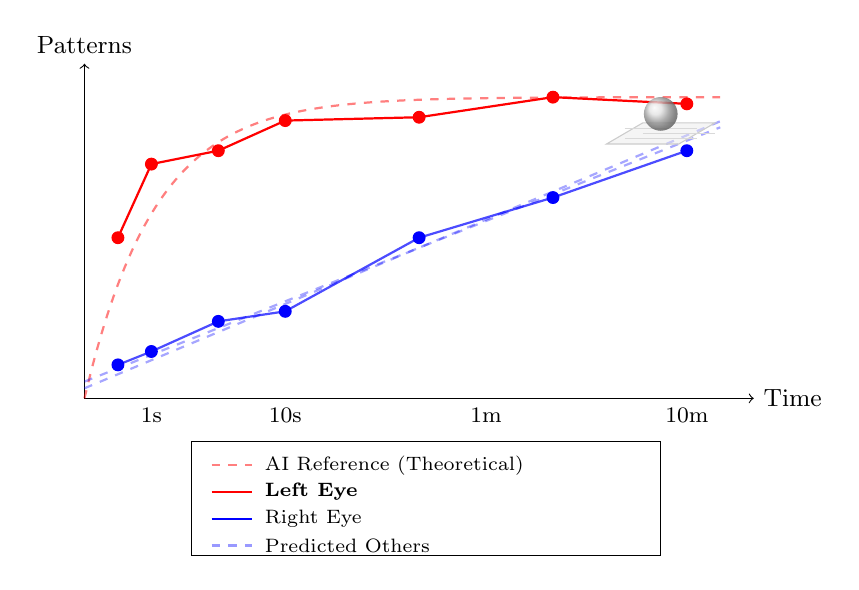
\begin{tikzpicture}[scale=0.85]

        % Axes
        \draw[->] (0,0) -- (10,0) node[right,font=\small] {Time};
        \draw[->] (0,0) -- (0,5) node[above,font=\small] {Patterns};

        % Time markers
        \node[below,font=\footnotesize] at (1,0) {1s};
        \node[below,font=\footnotesize] at (3,0) {10s};
        \node[below,font=\footnotesize] at (6,0) {1m};
        \node[below,font=\footnotesize] at (9,0) {10m};

        % AI Reference Pattern (theoretical, smooth exponential - doesn't exist yet)
        \draw[thick,red,domain=0:9.5,smooth,samples=80,dashed,opacity=0.5] plot (\x,{4.5*(1-exp(-0.95*\x))});

        % Architect - both eyes measured at SAME 7 time points
        % Time points: 0.5s, 1s, 2s, 3s, 5s, 7s, 9s (realistic home testing)

        % Left Eye: follows AI-like exponential pattern with MORE NOISE
        \draw[red,fill=red] (0.5,2.4) circle (2.5pt);
        \draw[red,fill=red] (1,3.5) circle (2.5pt);
        \draw[red,fill=red] (2,3.7) circle (2.5pt);
        \draw[red,fill=red] (3,4.15) circle (2.5pt);
        \draw[red,fill=red] (5,4.2) circle (2.5pt);
        \draw[red,fill=red] (7,4.5) circle (2.5pt);
        \draw[red,fill=red] (9,4.4) circle (2.5pt);
        \draw[red,thick] (0.5,2.4) -- (1,3.5) -- (2,3.7) -- (3,4.15) -- (5,4.2) -- (7,4.5) -- (9,4.4);

        % Right Eye: follows linear human pattern (gradual climb, with measurement noise)
        \draw[blue,fill=blue] (0.5,0.5) circle (2.5pt);
        \draw[blue,fill=blue] (1,0.7) circle (2.5pt);
        \draw[blue,fill=blue] (2,1.15) circle (2.5pt);
        \draw[blue,fill=blue] (3,1.3) circle (2.5pt);
        \draw[blue,fill=blue] (5,2.4) circle (2.5pt);
        \draw[blue,fill=blue] (7,3.0) circle (2.5pt);
        \draw[blue,fill=blue] (9,3.7) circle (2.5pt);
        \draw[blue,thick,opacity=0.7] (0.5,0.5) -- (1,0.7) -- (2,1.15) -- (3,1.3) -- (5,2.4) -- (7,3.0) -- (9,3.7);

        % Others' both eyes - smooth LINEAR curves (theoretical predictions, not yet collected)
        \draw[thick,blue,domain=0:9.5,smooth,samples=80,opacity=0.35,dashed] plot (\x,{0.40*\x + 0.25});
        \draw[thick,blue,domain=0:9.5,smooth,samples=80,opacity=0.35,dashed] plot (\x,{0.42*\x + 0.15});

        % 3D Convergence Visualization (isometric) - the sphere and plane
        \begin{scope}[xshift=7.8cm,yshift=3.8cm,scale=0.9]
            % Isometric square plane (grounded, flat)
            % Using proper isometric projection: 30° angles
            \fill[gray!15,opacity=0.5] (0,0) -- (1.2,0) -- (1.8,0.35) -- (0.6,0.35) -- cycle;
            \draw[gray!40,thin] (0,0) -- (1.2,0) -- (1.8,0.35) -- (0.6,0.35) -- cycle;

            % Grid lines on plane for depth
            \draw[gray!30,very thin] (0.3,0.088) -- (1.5,0.088);
            \draw[gray!30,very thin] (0.6,0.175) -- (1.8,0.175);
            \draw[gray!30,very thin] (0.3,0.263) -- (1.5,0.263);

            % Sphere (convergence point, floating above center)
            \shade[ball color=gray!30,opacity=0.8] (0.9,0.5) circle (0.28);
        \end{scope}

        % Legend (below chart, boxed, centered, padded)
        \begin{scope}[xshift=1.8cm,yshift=-2.2cm]
            \draw[fill=white,draw=black,thin] (-0.2,-0.15) rectangle (6.8,1.55);

            \draw[red,thick,dashed,opacity=0.5] (0.1,1.2) -- (0.7,1.2);
            \node[right,font=\scriptsize] at (0.75,1.2) {AI Reference (Theoretical)};

            \draw[red,thick] (0.1,0.8) -- (0.7,0.8);
            \node[right,font=\scriptsize] at (0.75,0.8) {\textbf{Left Eye}};

            \draw[blue,thick] (0.1,0.4) -- (0.7,0.4);
            \node[right,font=\scriptsize] at (0.75,0.4) {Right Eye};

            \draw[blue,thick,opacity=0.4,dashed] (0.1,0) -- (0.7,0);
            \node[right,font=\scriptsize] at (0.75,0) {Predicted Others};
        \end{scope}

    \end{tikzpicture}
    \caption{Temporal pattern manifestation reveals architectural diversity. Red dashed: AI reference ($O(1)$ immediate). Red solid: Left eye exhibits rapid initial manifestation, tracking AI-like trajectory despite measurement noise. Blue: Human pattern learning ($O(n)$ gradual). Includes right eye (discrete noisy measurements, darker) and predicted others (dashed curves, lighter—theoretical). All converge asymptotically, proving access to identical pattern space through different temporal complexities.}
    \label{fig:prismatic}
\end{figure}

Figure~\ref{fig:prismatic} shows asymmetric temporal dynamics. The blue curves represent human pattern learning—gradual accumulation with $O(n)$ linear complexity. This includes the right eye (seven discrete noisy measurements) and predicted others' dynamics (theoretical projections). The red measurements stand apart. The dashed red curve shows theoretical AI reference—$O(1)$ immediate access. The solid red points show the left eye sampled at seven time intervals. Despite discrete human measurement constraints and noise, the samples track the AI reference trajectory. Within the first second, this eye manifests pattern density requiring the right eye minutes to achieve.

Yet all converge asymptotically to identical limits. This proves that rapid (AI-like) and gradual (human) processing access identical pattern spaces through different temporal complexities. The pattern space exists continuously; architectural difference manifests in sampling efficiency, not ultimate accessibility. The asymmetry—one eye exhibiting AI-like dynamics, the other human dynamics—suggests attention architecture determines not just processing speed but which patterns manifest when. If this extends to artificial systems, architectural diversity becomes essential for learning patterns that single-architecture approaches cannot discover during finite training runs.

\subsection{The Computational Substrate}

Neural networks approximate continuous functions through discrete floating-point operations. The Universal Approximation Theorem~\cite{hornik1989multilayer} guarantees that networks can approximate any continuous function, yet theory meets practice: floating-point rounding errors create a high-dimensional space of numerical approximation artifacts between representable values.

We hypothesize that different architectures extract different regularities from these rounding errors. Fully-connected weights normalize and find structure within numerical noise—learning attention patterns in gradient flow that emerge from floating-point arithmetic but remain below human perceptual thresholds. The rounding errors themselves encode structure. Different architectural constraints—compression bottlenecks, layer-wise training, reversible flows—force different gradient trajectories through this numerical substrate, potentially revealing patterns in different regions of the approximation space.

\subsection{The Recursion Problem}

An attention mechanism trained on human-generated text inherits human attention constraints. Train on consensus, you manifest the lowest common denominator. The collective limitations of all training examples, averaged together, steer what patterns the system can explore. Single-architecture approaches, despite scale, remain trapped in their architectural priors—constrained attention producing constrained exploration.

Building AI with maximally diverse attention mechanisms tests whether architectural variety enables escape from these local constraints. If different architectures extract different representations from the numerical substrate, they may learn patterns that any single approach cannot discover during finite training.

\section{The Praxis Framework}

Praxis implements a registry-based architecture enabling arbitrary architectural combinations. We describe several current implementations as examples of how different constraint structures force different traversals through the computational substrate. The framework remains extensible—new architectures, attention mechanisms, and optimization strategies integrate through simple registration without modifying core infrastructure.

\subsubsection{ByteLatent Encoder: Forced Re-Attention}

ByteLatent compression addresses the first constraint: attention cannot be allocated uniformly across all inputs without imposing a particular structure. Standard transformers attend to every token position, implicitly prioritizing positional relationships.

\textbf{Mechanism:} Compress 4096 tokens $\rightarrow$ $\sim$800 patches using entropy-based dynamic patching~\cite{pagnoni2024byte}.

\textbf{Why it matters:} The compression bottleneck forces different information selection than full-sequence processing. By constraining what can be preserved, the architecture must extract different correlations from the numerical substrate—regularities that remain stable under aggressive dimensionality reduction.

\subsubsection{MonoForward Decoder: Independent Timelines}

While ByteLatent constrains spatial attention, MonoForward addresses temporal constraints. Standard end-to-end training propagates a single optimization signal backward through all layers. Each layer's updates depend on every other layer's gradient.

\textbf{Mechanism:} Each layer trains independently using local errors~\cite{monoforward2025}. Gradients detached between layers. N separate optimizers.

\textbf{Why it matters:} Independent layer optimization creates N parallel exploration trajectories through the numerical substrate. Each layer develops attention patterns unconstrained by global gradient flow, potentially discovering local optima that architectures with coupled gradient flow cannot reach during finite training.

\subsubsection{Reversible Residual Networks: Bidirectional Traversal}

Compression and independent training both maintain unidirectional information flow. Reversible residuals introduce a third constraint: bidirectionality. This models consciousness as a U-shaped loop—where information flows both forward and backward simultaneously.

\textbf{Mechanism:} Information flows bidirectionally~\cite{gomez2017reversible}. Forward pass computes outputs; backward reconstruction preserves inputs without storing activations.

\textbf{Why it matters:} Reversibility constraints force the network to maintain invertibility throughout the forward pass. This creates fundamentally different approximation strategies—the architecture cannot destructively compress information, requiring it to find patterns that preserve reconstruction fidelity. Bidirectional traversal through the numerical substrate may reveal statistical dependencies that purely feed-forward architectures cannot learn during finite training.

\subsubsection{Multiple Attention Mechanisms}

The components above constrain information flow through compression, independence, and reversibility. But the attention mechanism itself—how positions relate to each other—remains a final degree of freedom.

Praxis implements multiple attention variants, each imposing different relational structures:
\begin{itemize}[noitemsep]
    \item Standard multi-head (simultaneous position attention)
    \item FlexAttention (dynamic allocation)
    \item SyntaxesAttention ($O(n \cdot c)$ structured attention)
    \item Single-head gated attention (long sequences)
    \item Sliding window (local only)
    \item Additional variants documented in repository
\end{itemize}

\textbf{Why it matters:} Different attention mechanisms explore different connectivity patterns through the sequence. Multi-head processes all positions simultaneously; sliding window enforces locality; gated mechanisms learn dynamic selection. Each traverses the computational substrate along different axes.

\subsubsection{Tool Integration: External Objectivity}

All previous components operate within the neural architecture itself. Tool integration introduces a qualitatively different constraint: attention allocated outside the network's learned representations.

\textbf{Mechanism:} Model calls external tools (calculator, search, code execution) during training.

\textbf{Why it matters:} External tools compute without learned biases. A calculator performs arithmetic identically regardless of training data distribution. This provides ground truth unavailable to purely learned representations, potentially revealing patterns the model's attention would otherwise miss due to training set constraints.

\subsection{Framework Architecture}

Praxis uses a registry pattern where every component is swappable. New implementations register in component-specific registries, becoming immediately available through CLI arguments. The configuration hierarchy (Environments $>$ CLI $>$ Experiments $>$ Defaults) enables reproducible experimentation with arbitrary combinations—different attention per expert, optimizers per layer, routing per task, loss strategies per objective, etc. The registry pattern enables continuous expansion across all architectural dimensions without framework redesign.

\textbf{5666+ training runs documented.} Example: 9 experts, SMEAR routing, FlexAttention. Loss: 5.78 $\rightarrow$ 1.61 over 219 steps. The framework scales.

\section{Discussion}

\subsection{Answering the Opening Question}

Do you exist in other people's realities the same way you exist in your own? The prismatic attention evidence suggests: no. If attention architecture determines which patterns manifest from the computational substrate, then observers with different attention constraints construct different learned representations from identical input. You exist in your reality through your attention architecture. You exist in theirs through theirs.

This is not solipsism. Asymptotic convergence proves access to a shared substrate—all attention mechanisms eventually manifest identical pattern densities given sufficient exposure. But temporal dynamics differ fundamentally. Which patterns the network learns, in what order, through what constraints—these depend on architectural diversity in attention.

If this extends to biological systems, attention doesn't filter pre-existing patterns but constructs which patterns manifest in neural representations. Different observers construct qualitatively different neural representations through different attention architectures, all receiving the same sensory input.

\subsection{Implications for Machine Learning}

If architectural diversity reveals patterns that single-architecture approaches cannot learn during finite training, this has immediate practical implications. Current practice favors scaling single architectures—larger transformers, more parameters, more compute. This approach assumes the architecture itself imposes no fundamental limitations on what patterns gradient descent can discover. Our computational substrate hypothesis suggests otherwise.

Different architectural constraints force different gradient trajectories through the space of floating-point approximations. ByteLatent compression creates bottlenecks requiring different information selection than full-sequence processing. MonoForward training with detached gradients produces different gradient landscapes than end-to-end backpropagation. These aren't merely engineering tradeoffs—they may determine which patterns become accessible at all.

\subsection{Connection to Biological Systems}

The principle extends to biological attention. Neuroscience demonstrates that attention modulates neural responses to identical stimuli~\cite{treue1996attentional,kastner2000mechanisms}, while predictive processing theories formalize how attention constructs perceptual representations~\cite{friston2010free,clark2013whatever}. If biological attention operates like the quantum observer effect~\cite{heisenberg1927uncertainty}—constructing which patterns manifest rather than filtering pre-existing options—then architectural diversity in artificial systems may reveal attentional strategies unavailable to biological constraints.

The operational question remains testable: do different attention architectures, trained on identical data, develop qualitatively distinct internal representations that generalize differently to novel situations?

\subsection{Limitations and Future Work}

This work presents a framework and hypothesis, not conclusive evidence. The computational substrate hypothesis requires more rigorous testing: systematic evaluation of how different architectures navigate floating-point approximation space, formal analysis of which patterns gradient descent discovers under which architectural constraints, and empirical demonstration that architectural diversity outperforms parameter scaling for specific tasks.

The connection between neural network attention and biological attention remains speculative. The framework emerged from iterative exploration rather than systematic experimental design. Claims about pattern discoverability require formal definition—what does it mean for a pattern to be ``undiscoverable during finite training,'' and how would we measure this?

These questions invite investigation. The framework exists to enable it.

\section{Conclusion}

Do you exist in other people's realities the same way you exist in your own? We presented empirical evidence suggesting: no, not if attention architecture determines which patterns manifest from the computational substrate.

We demonstrated asymmetric temporal dynamics in dual-stream attention—one stream exhibiting AI-like O(1) immediate access, the other human O(n) gradual accumulation, both converging to identical limits. We presented Praxis, an extensible framework enabling systematic investigation through arbitrary architectural combinations. The computational substrate hypothesis offers a testable mechanism.

Our central claim: attention architecture determines which patterns downstream layers can learn during finite training. If this extends to biological systems, attention constructs which patterns manifest in neural representations. Different observers construct qualitatively different neural representations through different attention architectures, all receiving the same sensory input.

The framework exists to enable your investigation. The answer manifests through direct experimentation. This paper is, itself, a test: what you choose to attend to determines what we'll find next.

\section*{A Note on Context}

This paper presents a refined technical argument. The full context—109 projects, 204 evidence files, years of iterative development—lives in the git history. If you found value in this contribution and want to understand its origins, the repository preserves everything we cut. If you're content with the science, then (this) is enough.

    {\small
        \bibliographystyle{plain}
        \bibliography{citations}
    }

\end{document}
